% -*- TeX -*- -*- UK -*- -*- Soft -*-

\chapter{Bayesian Inference Problem, MCMC and Variational Inference}
\label{chap:BayesianInferenceIroblemMCMCandVariationalInference}

This chapter is a verbatim copy of a blog \cite{JosephRoccaBayes2019} by Joseph Rocca.

\textit{Overview of the Bayesian inference problem in statistics.}

\section{Introduction}

Bayesian inference is a major problem in statistics that is also encountered in many machine learning methods. For example, Gaussian mixture models, for classification, or Latent Dirichlet Allocation, for topic modelling, are both graphical models requiring to solve such a problem when fitting the data.

Meanwhile, it can be noticed that Bayesian inference problems can sometimes be very difficult to solve depending on the model settings (assumptions, dimensionality, $\ldots$). In large problems, exact solutions require, indeed, heavy computations that often become intractable and some approximation techniques have to be used to overcome this issue and build fast and scalable systems.

In this post we will discuss the two main methods that can be used to tackle the Bayesian inference problem: Markov Chain Monte Carlo (MCMC), that is a sampling based approach, and Variational Inference (VI), that is an approximation based approach.

\section{Outline}

In the first section we will discuss the Bayesian inference problem and see some examples of classical machine learning applications in which this problem naturally appears. Then in the second section we will present globally MCMC technique to solve this problem and give some details about two MCMC algorithms: Metropolis-Hasting and Gibbs Sampling. Finally in the third section we will introduce Variational Inference and see how an approximate solution can be obtained following an optimisation process over a parametrised family of distributions.

Notice  that in this post $p(.)$ is used to denote either probability, probability density or probability distribution depending on the context.

\section{The Bayesian inference problem}

In this section we present the Bayesian inference problem and discuss some computational difficulties before giving the example of Latent Dirichlet Allocation, a concrete machine learning technique of topic modelling in which this problem is encountered.

\subsection{What is inference?}

Statistical inference consists in \textbf{learning about what we do not observe based on what we observe}. In other words, it is the process of drawing conclusions such as punctual estimations, confidence intervals or distribution estimations about some latent variables (often causes) in a population, based on some observed variables (often effects) in this population or in a sample of this population.

In particular, \textbf{Bayesian inference} is the process of producing statistical inference taking a Bayesian point of view. In short, the Bayesian paradigm is a statistical/probabilistic paradigm in which a prior knowledge, modelled by a probability distribution, is updated each time a new observation, whose uncertainty is modelled by another probability distribution, is recorded. The whole idea that rules the Bayesian paradigm is embed in the so called Bayes theorem that expresses the relation between the updated knowledge (the "posterior"), the prior knowledge (the "prior") and the knowledge coming from the observation (the "likelihood").

A classical example is the \textbf{Bayesian inference of parameters}. Let's assume a model where data $x$ are generated from a probability distribution depending on an unknown parameter $\theta$. Let's also assume that we have a prior knowledge about the parameter $\theta$ that can be expressed as a probability distribution $p(\theta)$. Then, when data $x$ are observed, we can update the prior knowledge about this parameter using the Bayes theorem as follows


\begin{figure*}[h]
    \centering
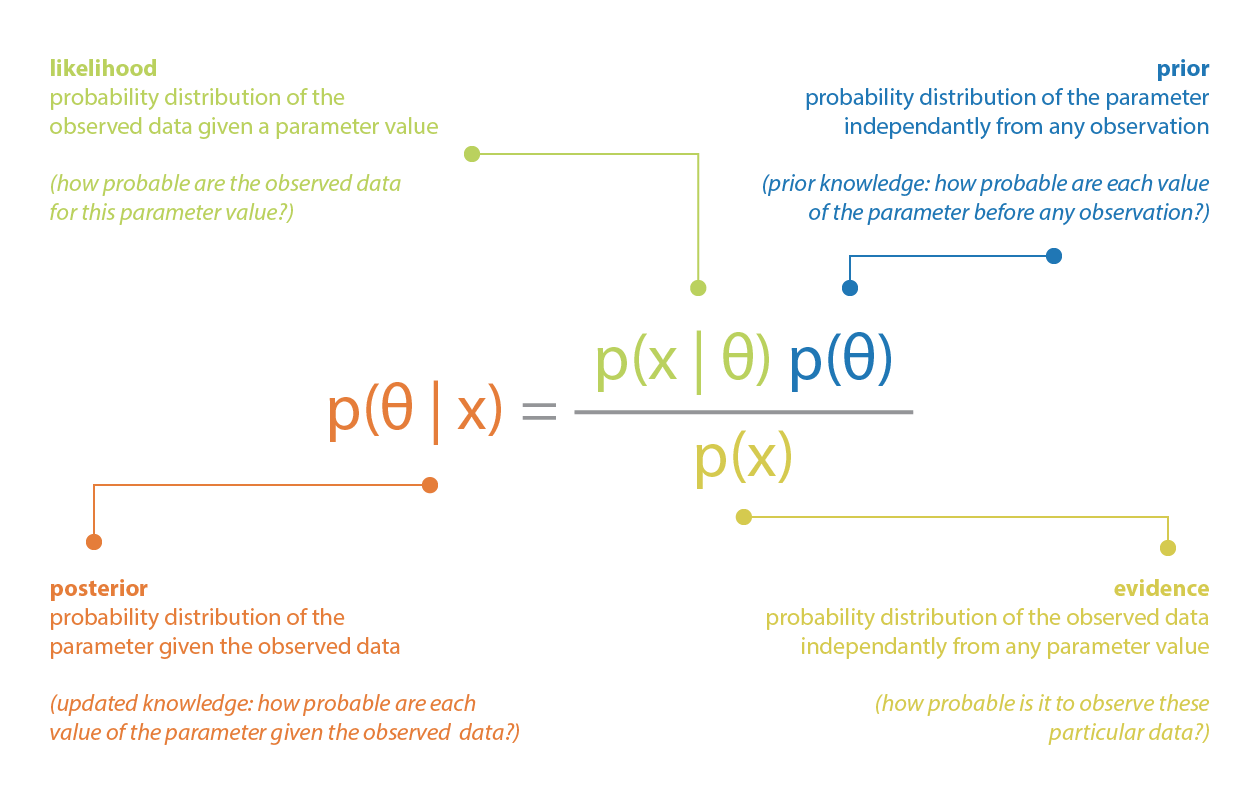
\includegraphics[width=0.8\textwidth]{pic/p05c07-snip01.png}
    \caption{Illustration of the Bayes theorem applied to the inference of a parameter given observed data}
    \label{fig:p05c07-snip01}
\end{figure*}


\subsection{Computational difficulties}

The Bayes theorem tells us that the computation of the posterior requires three terms: a prior, a likelihood and an evidence. The first two can be expressed easily as they are part of the assumed model (in many situation, the prior and the likelihood are explicitly known). However, the third term, that is a normalisation factor, requires to be computed such that

\begin{equation}p(x)=\int_{\theta} p(x | \theta) p(\theta) d \theta\end{equation}

Although in low dimension this integral can be computed without too much difficulties, \textbf{it can become intractable in higher dimensions}. In this last case, the exact computation of the posterior distribution is practically infeasible and some approximation techniques have to be used to get solutions to problems that require to know this posterior (such as mean computation, for example).

We can notice that some other computational difficulties can arise from Bayesian inference problem such as, for example, combinatorics problems when some variables are discrete. Among the approaches that are the most used to overcome these difficulties we find \textbf{Markov Chain Monte Carlo} and \textbf{Variational Inference} methods. Later in this post, we will describe these two approaches focusing especially on the "normalisation factor problem" but one should keep in mind that these methods can also be precious when facing other computational difficulties related to Bayesian inference.

In order to make things a lit bit more general for the upcoming sections, we can observe that, as $x$ is supposed to be given and can, so, be treated as a parameter, we face a situation where we have a probability distribution on $\theta$ defined up to a normalisation factor

\begin{equation}\pi_{x}(\theta) \equiv p(\theta | x) \propto p(x | \theta) p(\theta) \equiv g_{x}(\theta)\end{equation}

Before describing MCMC and VI in the next two sections, let's give a concrete example of Bayesian inference problem in machine learning with Latent Dirichlet Allocation.

\subsection{Example}

Bayesian inference problem naturally appears, for example, in machine learning methods that assume a probabilistic graphical model and where, given some observations, we want to recover latent variables of the model. In topic modelling, the \textbf{Latent Dirichlet Allocation (LDA)} method defines such a model for the description of texts in a corpus. Thus, given the full corpus vocabulary of size $V$ and a given number of topics $T$, the model assumes:

\begin{itemize}
    \item     there exists, for each topic, a "topic-word" probability distribution over the vocabulary (with a Dirichlet prior assumed)
    \item     there exists, for each document, a "document-topic" probability distribution over the topics (with another Dirichlet prior assumed)
    \item     each word in a document have been sampled such that, first, we have sampled a topic from the "document-topic" distribution of the document and, second, we have sampled a word from the "topic-word" distribution attached to the sampled topic
\end{itemize}


The purpose of the method, whose name comes from the Dirichlet priors assumed in the model, is then to infer the latent topics in the observed corpus as well as the topic decomposition of each documents. Even if we won't dive into details of LDA, we can say very roughly, denoting $w$ the vector of words in the corpus and $z$ the vector of topics associated to these words, that we want to infer $z$ based on the observed $w$ in a Bayesian way:

\begin{equation}p(z | w)=\frac{p(w | z) p(z)}{p(w)}=\frac{p(w | z) p(z)}{\int_{z} p(w | z) p(z) d z}\end{equation}

Here, beyond the fact that the normalisation factor is absolutely intractable due to a huge dimensionality, we face a combinatoric challenge (as some variables of the problem are discrete) that require to use either MCMC or VI to get an approximate solution. The reader interested by topic modelling and its specific underlying Bayesian inference problem can take a look at this reference paper \cite{Blei2003a}  on LDA.


\begin{figure*}[h]
    \centering
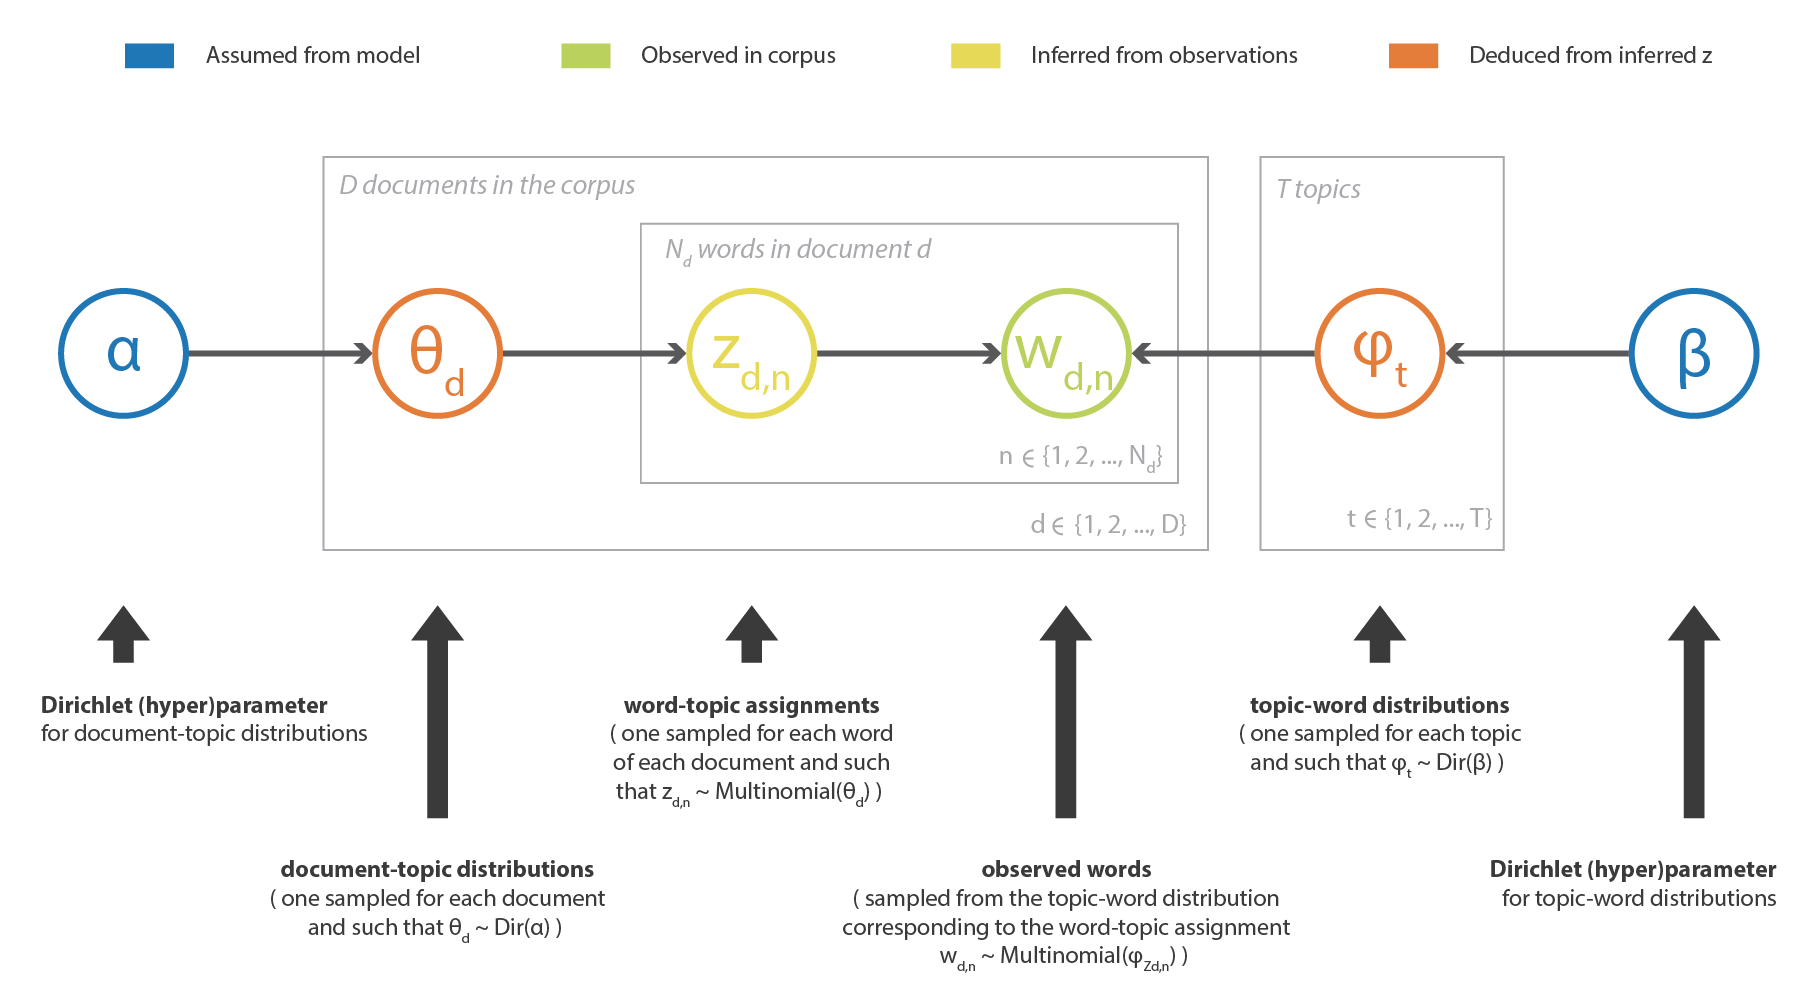
\includegraphics[width=\textwidth]{pic/p05c07-snip02.png}
    \caption{Illustration of the Latent Dirichlet Allocation method}
    \label{fig:p05c07-snip02}
\end{figure*}


\section{Markov Chains Monte Carlo (MCMC)}

As we mentioned before, one of the main difficulty faced when dealing with a Bayesian inference problem comes from the normalisation factor. In this section we describe \textbf{MCMC sampling methods} that constitute a possible solution to overcome this issue as well as some others computational difficulties related to Bayesian inference.

\subsection{The sampling approach}

The idea of sampling methods is the following. Let's assume first that we have a way (MCMC) to \textbf{draw samples from a probability distribution defined up to a factor}. Then, instead of trying to deal with intractable computations involving the posterior, we can get samples from this distribution (using only the not normalised part definition) and use these samples to compute various punctual statistics such as mean and variance or even to approximate the distribution by Kernel Density Estimation.

Contrarily to VI methods described in the next section, \textbf{MCMC approaches assume no model} for the studied probability distribution (the posterior in the Bayesian inference case). As a consequence, these methods have a low bias but a high variance and it implies that results are most of the time more costly to obtain but also more accurate than the one we can get from VI.

To conclude this subsection, we outline once more the fact that this sampling process we just described is not constrained to the Bayesian inference of posterior distribution and can also, more generally, be used in any situation where a probability distribution is defined up to its normalisation factor.


\begin{figure*}[h]
    \centering
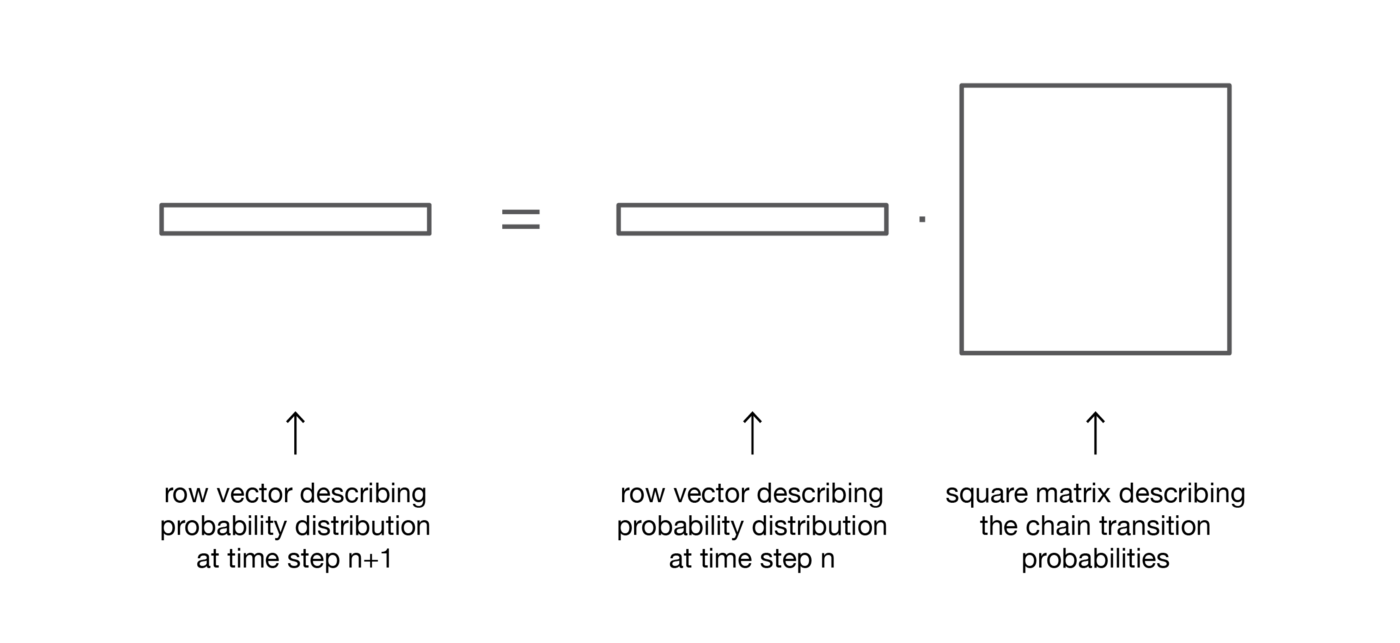
\includegraphics[width=\textwidth]{pic/p05c07-snip03.png}
    \caption{Illustration of the sampling approach (MCMC)}
    \label{fig:p05c07-snip03}
\end{figure*}


\subsection{The idea of MCMC}

In statistics, \textbf{Markov Chain Monte Carlo algorithms are aimed at generating samples from a given probability distribution}. The "Monte Carlo" part of the method's name is due to the sampling purpose whereas the "Markov Chain" part comes from the way we obtain these samples (we refer the reader to our introductory post on Markov Chains \cite{JosephRoccaMarkovChains2019}), see Chapter~\ref{chap:IntroductiontoMarkovChains}.


In order to produce samples, the idea is to set up a Markov Chain whose stationary distribution is the one we want to sample from. Then, we can simulate a random sequence of states from that Markov Chain that is long enough to (almost) reach the steady state and then keep some generated states as our samples.

Among the random variables generation techniques, MCMC is a pretty advanced kind of methods (we already discussed an other method in our post about GANs) that makes possible to \textbf{get samples from a very difficult probability distribution potentially defined only up to a multiplicative constant}. The counter-intuitive fact that we can obtain, with MCMC, samples from a distribution not well normalised comes from the specific way we define the Markov Chain that is not sensitive to these normalisation factor.


\begin{figure*}[h]
    \centering
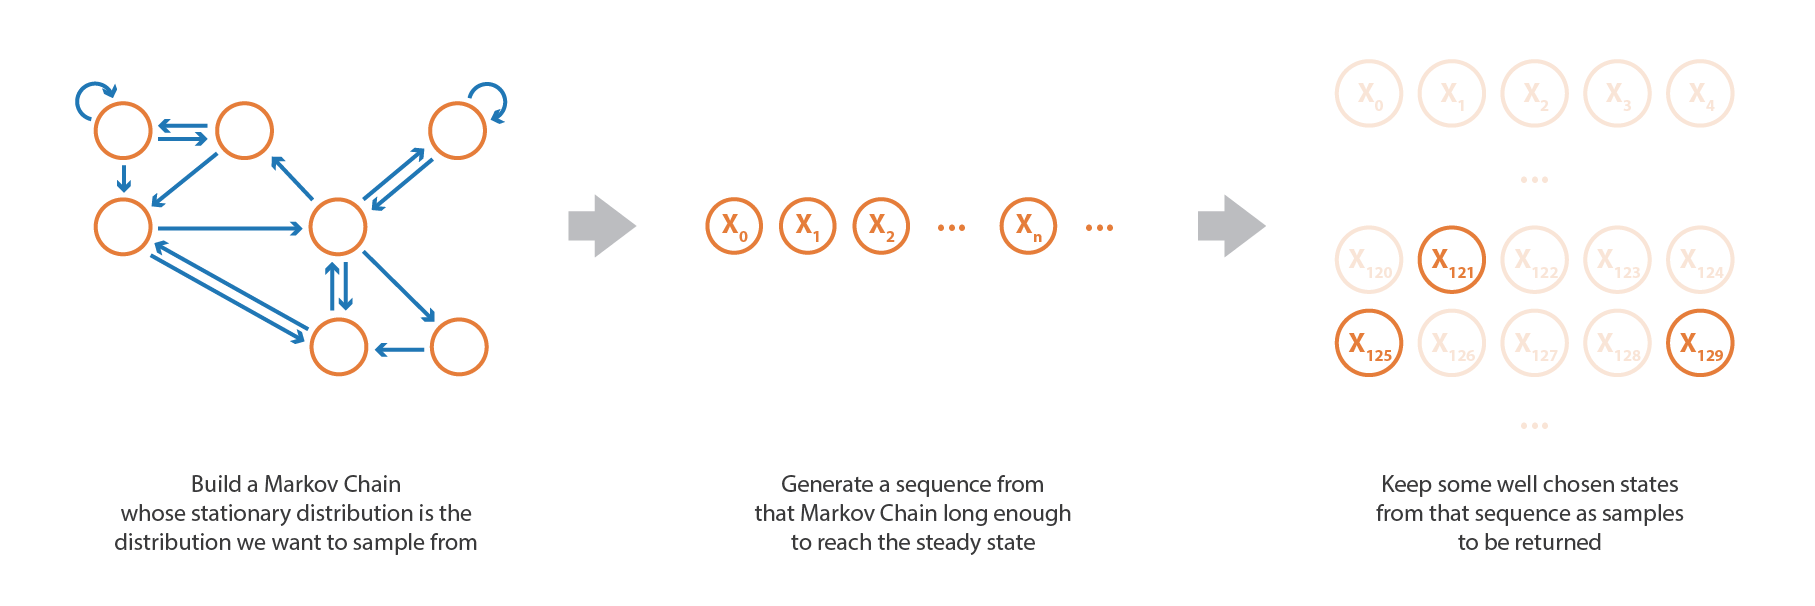
\includegraphics[width=\textwidth]{pic/p05c07-snip04.png}
    \caption[The Markov Chain Monte Carlo approach is aimed at generating samples]{The Markov Chain Monte Carlo approach is aimed at generating samples from a difficult probability distribution that can be defined up to a factor}
    \label{fig:p05c07-snip04}
\end{figure*}


\subsection{Definition of the Markov Chain}

The whole MCMC approach is based on the ability to \textbf{build a Markov Chain whose stationary distribution is the one we want to sample from}. In order to do so, Metropolis-Hasting and Gibbs Sampling algorithms both use a particular property of Markov Chains: reversibility.

A Markov Chain over a state space E with transition probabilities denoted by
\begin{equation}k(\alpha, \beta) \equiv p\left(X_{n+1}=\beta | X_{n}=\alpha\right)\end{equation}
is said to be reversible if there exists a probability distribution $\gamma$ such that
\begin{equation}k(\alpha, \beta) \gamma(\alpha)=k(\beta, \alpha) \gamma(\beta) \quad \forall \alpha, \beta \in E\end{equation}
For such Markov Chain, we can easily verify that we have
\begin{equation}\int_{\beta \in E} k(\beta, \alpha) \gamma(\beta) d \beta=\int_{\beta \in E} k(\alpha, \beta) \gamma(\alpha) d \beta=\gamma(\alpha)\end{equation}
and, then, $\gamma$ is a stationary distribution (the only one if the Markov Chain is irreducible).

Let's now assume that the probability distribution $\pi$ we want to sample from is only defined up to a factor
\begin{equation}\pi(.)=C \times g(.) \propto g(.)\end{equation}
(where $C$ is the unknown multiplicative constant). We can notice that the following equivalence holds
\begin{equation}\begin{aligned}
& k(\alpha, \beta) \pi(\alpha) &=k(\beta, \alpha) \pi(\beta) & & \forall \alpha, \beta \in E \\
\Longleftrightarrow & k(\alpha, \beta) g(\alpha) &=k(\beta, \alpha) g(\beta) & & \forall \alpha, \beta \in E
\end{aligned}\end{equation}
and, then, a Markov Chain with transition probabilities $k(.,.)$ defined to verify the last equality will have, as expected, $\pi$ as stationary distribution. Thus, we can define a Markov Chain that have for stationary distribution a probability distribution $\pi$ that can't be explicitly computed.

\subsection{The Gibbs Sampling transitions}

Let's assume that the Markov Chain we want to define is $D$-dimensional, such that
\begin{equation}X_{n}=\left(X_{n, 1}, X_{n, 2}, \dots, X_{n, D}\right)\end{equation}
The \textbf{Gibbs Sampling method} is based on the assumption that, even if the joint probability is intractable, the conditional distribution of a single dimension given the others can be computed. Based on this idea, transitions are defined such that, at iteration $n+1$, the next state to be visited is given by the following process.

First we randomly choose an integer d among the $D$ dimensions of $X_n$. Then we sample a new value for that dimension according to the corresponding conditional probability given that all the other dimensions are kept fixed:
\begin{eqnarray}
d 
&\sim& \text {Uniform}(\{1,2, \ldots, D\}) \quad, \nonumber \\
&&\quad X_{(n+1), j}=X_{n, j} \quad \forall j \neq d \quad \text { and } \nonumber \\
&&\quad X_{(n+1), d} \sim \pi_{d}\left(\cdot | X_{n, \neg d}\right)\nonumber
\end{eqnarray}
where
\begin{eqnarray}
\pi_{d}\left(\cdot | X_{n, \neg d}\right)
&=&\frac{\pi\left(X_{n, 1}, \ldots, X_{n,(d-1)}, \cdot, X_{n,(d+1)}, \ldots, X_{n, D}\right)}{\int_{u} \pi\left(X_{n, 1}, \ldots, X_{n,(d-1)}, u, X_{n,(d+1)}, \ldots, X_{n, D}\right) d u}\nonumber \\
&=&\frac{g\left(X_{n, 1}, \dots, X_{n,(d-1)}, \cdot, X_{n,(d+1)}, \dots, X_{n, D}\right)}{\int_{u} g\left(X_{n, 1}, \dots, X_{n,(d-1)}, u, X_{n,(d+1)}, \dots, X_{n, D}\right) d \imath}\nonumber
\end{eqnarray}
is the conditional distribution of the d-th dimension given all the other dimensions.

Formally, if we denote
%\begin{equation}\alpha \underset{d}^{\beta} \Longleftrightarrow \alpha_{i}=\beta_{i} \quad \forall i \neq d\end{equation}
\begin{equation}
\alpha \underset{d}{\sim}{\beta} \Longleftrightarrow 
\alpha_{i}=\beta_{i} 
\quad \forall i \neq d
\end{equation}
the transition probabilities can then be written
\begin{equation}k(\alpha, \beta)=\left\{\begin{array}{ll}
\frac{1}{D} \frac{g(\beta)}{\int_{\gamma \underset{d}{\sim}\alpha} g(\gamma) d \gamma} & \text { if } \beta \underset{d}{\sim} \alpha \\
0 & \text { otherwise }
\end{array} \quad \forall \beta \neq \alpha\right.\end{equation}
and, so, the local balance is verified as expected with, for the only non-trivial case,
\begin{equation}g(\alpha) k(\alpha, \beta)
=\frac{1}{D} \frac{g(\alpha) g(\beta)}{\int_{\gamma \underset{d}{\sim}\alpha} g(\gamma) d \gamma}
=\frac{1}{D} \frac{g(\beta) g(\alpha)}{\int_{\gamma \underset{d}{\sim}\beta} g(\gamma) d \gamma}=g(\beta) k(\beta, \alpha)\end{equation}

\subsection{The Metropolis-Hasting transitions}

Sometimes even conditional distributions involved in Gibbs methods are far too complex to be obtained. In such cases, \textbf{Metropolis-Hasting} can then be used. For this, we start by defining a side transition probability $h(.,.)$ that will serve at suggesting transitions. Then, at iteration $n+1$, the next state to be visited by the Markov Chain is defined by the following process. We first draw a "suggested transition" $x$ from $h$ and compute a related probability $r$ to accept it:
\begin{equation}\begin{aligned}
&x \sim h\left(X_{n}, .\right)\\
&\text { and } \quad r=\min \left(1, \frac{g(x) h\left(x, X_{n}\right)}{g\left(X_{n}\right) h\left(X_{n}, x\right)}\right)
\end{aligned}\end{equation}
Then the effective transition is chosen such that
\begin{equation}X_{n+1}=\left\{\begin{array}{ll}
x & \text { with probability } r \\
X_{n} & \text { with probability } 1-r
\end{array}\right.\end{equation}
Formally, the transition probabilities can then be written
\begin{equation}k(\alpha, \beta)=h(\alpha, \beta) \min \left(1, \frac{g(\beta) h(\beta, \alpha)}{g(\alpha) h(\alpha, \beta)}\right) \quad \forall \beta \neq \alpha\end{equation}
and, so, the local balance is verified as expected
\begin{equation}\begin{aligned}
g(\alpha) k(\alpha, \beta) &=g(\alpha) h(\alpha, \beta) \min \left(1, \frac{g(\beta) h(\beta, \alpha)}{g(\alpha) h(\alpha, \beta)}\right)=\min (g(\alpha) h(\alpha, \beta), g(\beta) h(\beta, \alpha)) \\
&=g(\beta) h(\beta, \alpha) \min \left(1, \frac{g(\alpha) h(\alpha, \beta)}{g(\beta) h(\beta, \alpha)}\right)=g(\beta) k(\beta, \alpha)
\end{aligned}\end{equation}

\subsection{The sampling process}

Once our Markov Chain has been defined, we can simulate a random sequence of states (randomly initialised) and keep some of them chosen such as to obtain samples that, both, follow the targeted distribution and are independent.

First, in order to have samples that (almost) follow the targeted distribution, we need to only consider states far enough from the beginning of the generated sequence to have almost reach the steady state of the Markov Chain (the steady state being, in theory, only asymptotically reached). Thus, the first simulated states are not usable as samples and we call this phase required to reach stationarity the burn-in time. Notice that, in practice it is pretty difficult to know how long this burn-in time has to be.

Second, in order to have (almost) independent samples, we can't keep all the successive states of the sequence after the burn-in time. Indeed, the Markov Chain definition implies a strong correlation between two successive states and we then need to keep as samples only states that are far enough from each other to be considered as almost independent. In practice, the lag required between two states to be considered as almost independent can be estimated through the analysis of the autocorrelation function (only for numeric values).

So, in order to get our independent samples that follow the targeted distribution, we keep states from the generated sequence that are separated from each other by a lag L and that come after the burn-in time B. Thus, if the successive states of the Markov Chain are denoted
\begin{equation}\left(X_{n}\right)_{n \geq 0}=X_{0}, X_{1}, X_{2}, \dots\end{equation}
we only keep as our samples the states
\begin{equation}X_{B}, X_{B+L}, X_{B+2 L}, X_{B+3 L}, \dots\end{equation}

\begin{figure*}[h]
    \centering
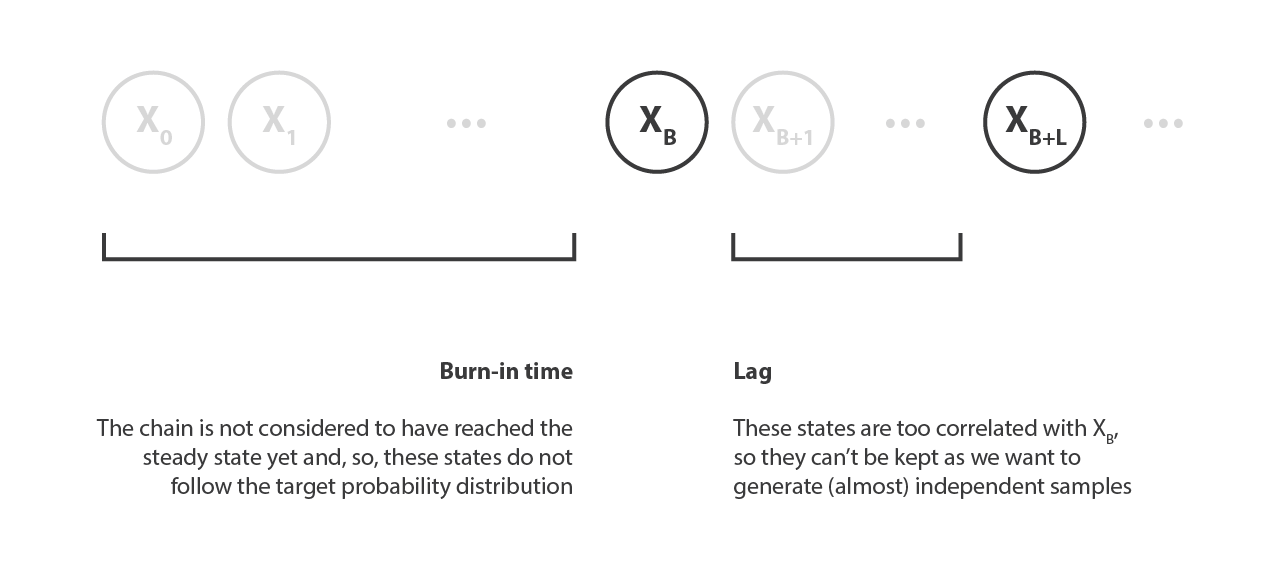
\includegraphics[width=\textwidth]{pic/p05c07-snip05.png}
    \caption{MCMC sampling requires to consider both a burn-in time and a lag}
    \label{fig:p05c07-snip05}
\end{figure*}


\section{Variational Inference (VI)}

Another possible way to overcome computational difficulties related to inference problem is to use Variational Inference methods that consist in finding the best approximation of a distribution among a parametrised family. In order to find this best approximation, we follow an optimisation process (over the family parameters) that only require the targeted distribution to be defined up to a factor.

\subsection{The approximation approach}

VI methods consist in searching for the best approximation of some complex target probability distribution among a given family. More specifically, the idea is to define a parametrised family of distributions and to optimise over the parameters to obtain the closest element to the target with respect to a well defined error measure.

Let's still consider our probability distribution $\pi$ defined up to a normalisation factor $C$:
\begin{equation}\pi(.)=C \times g(.) \propto g(.)\end{equation}
Then, in more mathematical terms, if we denote the parametrised family of distributions
\begin{equation}\mathcal{F}_{\Omega}=\left\{f_{\omega} ; \omega \in \Omega\right\} \quad \Omega \equiv \text { set of possible parameters }\end{equation}
and we consider the error measure $E(p,q)$ between two distributions $p$ and $q$, we search for the best parameter such that
\begin{equation}\omega^{*}=\underset{\omega \in \Omega}{\arg \min } E\left(f_{\omega}, \pi\right)\end{equation}
If we can solve this minimisation problem without having to explicitly normalise $\pi$, we can use $f_{\omega*}$ as an approximation to estimate various quantities instead of dealing with intractable computations. The optimisation problem implied by variational inference approaches is, indeed, supposed to be much simpler to handle than issues coming from direct computations (normalisation, combinatorics, $\ldots$).

Contrarily to sampling approaches, a model is assumed (the parametrised family), implying a bias but also a lower variance. In general VI methods are less accurate that MCMC ones but produce results much faster: these methods are better adapted to big scale, very statistical, problems.


\begin{figure*}[h]
    \centering
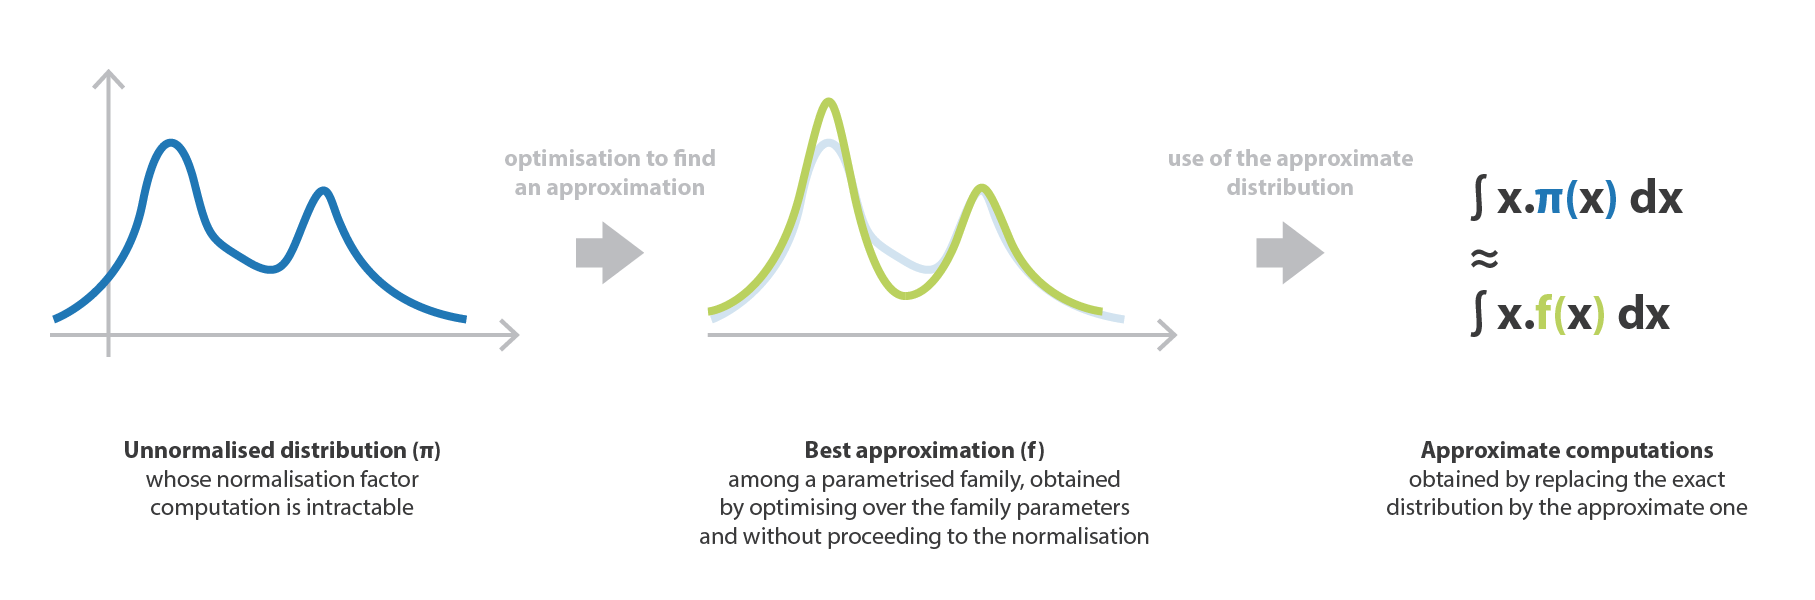
\includegraphics[width=\textwidth]{pic/p05c07-snip06.png}
    \caption{Illustration of the approximation approach (Variational Inference)}
    \label{fig:p05c07-snip06}
\end{figure*}

\subsection{Family of distribution}

The first thing we need to set up is the parametrised family of distributions that defines the space in which we search for our best approximation.

The choice of the family defines a model that control both the bias and the complexity of the method. If we assume a pretty restrictive model (simple family) then we have a high bias but the optimisation process is simple. On the contrary, if we assume a pretty free model (complex family) the bias is much lower but the optimisation is harder (if not intractable). Thus, we have to find the right balance between a family that is complex enough to ensure a good quality of the final approximation and a family that is simple enough to make the optimisation process tractable. We should keep in mind that if no distribution in the family is close to the target distribution, then even the best approximation can give poor results.

The mean-field variational family is a family of probability distributions where all the components of the considered random vector are independent. Distributions from this family have product densities such that each independent component is governed by a distinct factor of the product. Thus, a distribution that belongs to the mean-field variational family has a density that can be written
\begin{equation}f(z)=\prod_{j=1}^{m} f_{j}\left(z_{j}\right)\end{equation}
where we have assumed a $m$-dimensional random variable $z$. Notice that, even if it has been omitted in the notation, all the densities $f_j$ are parametrised. So, for example, if each density $f_j$ is a Gaussian with both mean and variance parameters, the global density $f$ is then defined by a set of parameters coming from all the independent factors and the optimisation is done over this entire set of parameters.


\begin{figure*}[h]
    \centering
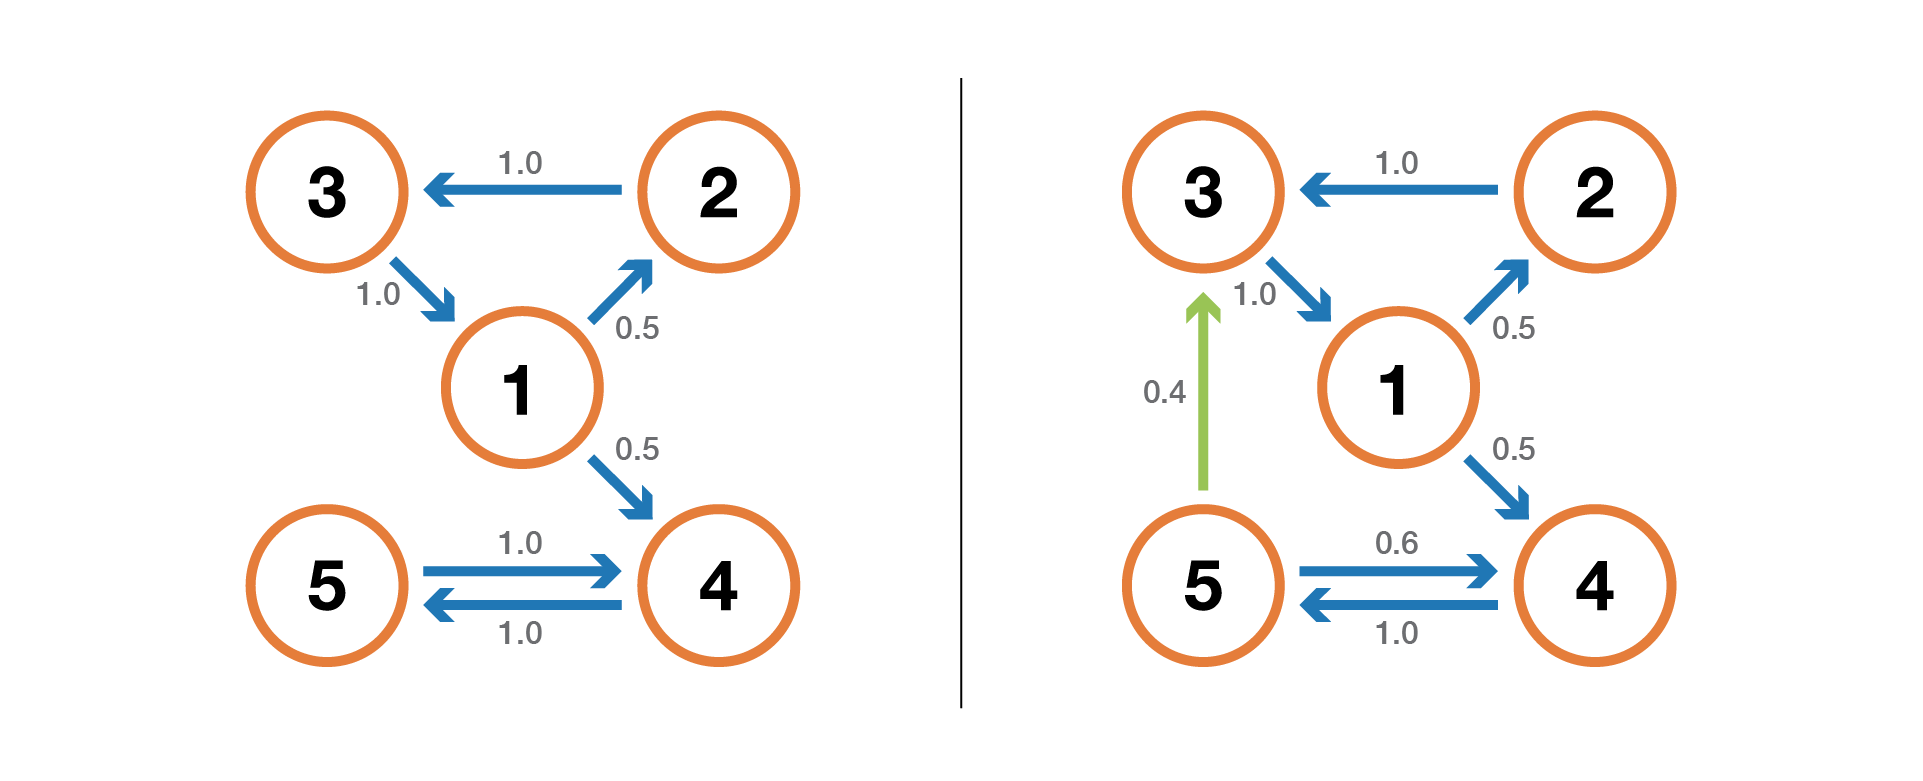
\includegraphics[width=\textwidth]{pic/p05c07-snip07.png}
    \caption[The choice of the family in variational inference sets]{The choice of the family in variational inference sets both the difficulty of the optimisation process and the quality of the final approximation}
    \label{fig:p05c07-snip07}
\end{figure*}

\subsection{Kullback-Leibler divergence}

Once the family has been defined, one major question remains: how to find, among this family, the best approximation of a given probability distribution (explicitly defined up to its normalisation factor)? Even if the best approximation obviously depends on the nature of the error measure we consider, it seems pretty natural to assume that the minimisation problem should not be sensitive to normalisation factors as we want to compare masses distributions more than masses themselves (that have to be unitary for probability distributions).

So, let's now define the Kullback-Leibler (KL) divergence and see that this measure makes the problem insensitive to normalisation factors. If $p$ and $q$ are two distributions, the KL divergence is defined as follows
\begin{equation}K L(p, q)=\mathbb{E}_{z \sim p}[\log p(z)]-\mathbb{E}_{z \sim p}[\log q(z)]\end{equation}
From that definition, we can pretty easily see that we have
\begin{equation}K L\left(f_{\omega}, C g\right)=\mathbb{E}_{z \sim f_{\omega}}\left[\log f_{\omega}(z)\right]-\mathbb{E}_{z \sim f_{\omega}}[\log (C g(z))]=\mathbb{E}_{z \sim f_{\omega}}\left[\log f_{\omega}(z)\right]-\mathbb{E}_{z \sim f_{\omega}}[\log g(z)]-\log C\end{equation}
which implies the following equality for our minimisation problem
\begin{equation}\omega^{*}=\underset{\omega \in \Omega}{\arg \min } K L\left(f_{\omega}, \pi\right)=\underset{\omega \in \Omega}{\arg \min } K L\left(f_{\omega}, C g\right)=\underset{\omega \in \Omega}{\arg \min } K L\left(f_{\omega}, g\right)\end{equation}
Thus, when choosing KL divergence as our error measure, the optimisation process is not sensitive to multiplicative coefficients and we can search for the best approximation among our parametrised family of distributions without having to compute the painful normalisation factor of the targeted distribution, as it was expected.

Finally, as a side fact, we can conclude this subsection by noticing for the interested readers that the KL divergence is the cross-entropy minus the entropy and has a nice interpretation in information theory.

\subsection{Optimisation process and intuition}

Once both the parametrised family and the error measure have been defined, we can initialise the parameters (randomly or according to a well defined strategy) and proceed to the optimisation. Several classical optimisation techniques can be used such as gradient descent or coordinate descent that will lead, in practice, to a local optimum.

In order to better understand this optimisation process, let's take an example and go back to the specific case of the Bayesian inference problem where we assume a posterior such that
\begin{equation}p(z | x) \propto p(x | z) p(z)=p(x, z)\end{equation}
In this case, if we want to get an approximation of this posterior using variational inference, we have to solve the following optimisation process (assuming the parametrised family defined and KL divergence as error measure)
\begin{equation}\begin{aligned}
\omega^{*} &=\underset{\omega \in \Omega}{\arg \min } K L\left(f_{\omega}(z), p(z | x)\right) \\
&=\underset{\omega \in \Omega}{\arg \min } K L\left(f_{\omega}(z), p(x, z)\right) \\
&=\underset{\omega \in \Omega}{\arg \max }\left(-K L\left(f_{\omega}(z), p(x, z)\right)\right) \\
&=\underset{\omega \in \Omega}{\arg \max }\left(\mathbb{E}_{z \sim f_{\omega}}[\log p(z)]+\mathbb{E}_{z \sim f_{\omega}}[\log p(x | z)]-\mathbb{E}_{z \sim f_{\omega}}\left[\log f_{\omega}(z)\right]\right) \\
&=\underset{\omega \in \Omega}{\arg \max }\left(\mathbb{E}_{z \sim f_{\omega}}[\log p(x | z)]-K L\left(f_{\omega}, p(z)\right)\right)
\end{aligned}\end{equation}
The last equality helps us to better understand how the approximation is encouraged to distribute its mass. The first term is the expected log-likelihood that tends to adjust parameters so that to place the mass of the approximation on values of the latent variables $z$ that explain the best the observed data. The second term is the negative KL divergence between the approximation and the prior that tends to adjust the parameters in order to make the approximation be close to the prior distribution. Thus, this objective function expresses pretty well the usual prior/likelihood balance.

\begin{figure*}[h]
    \centering
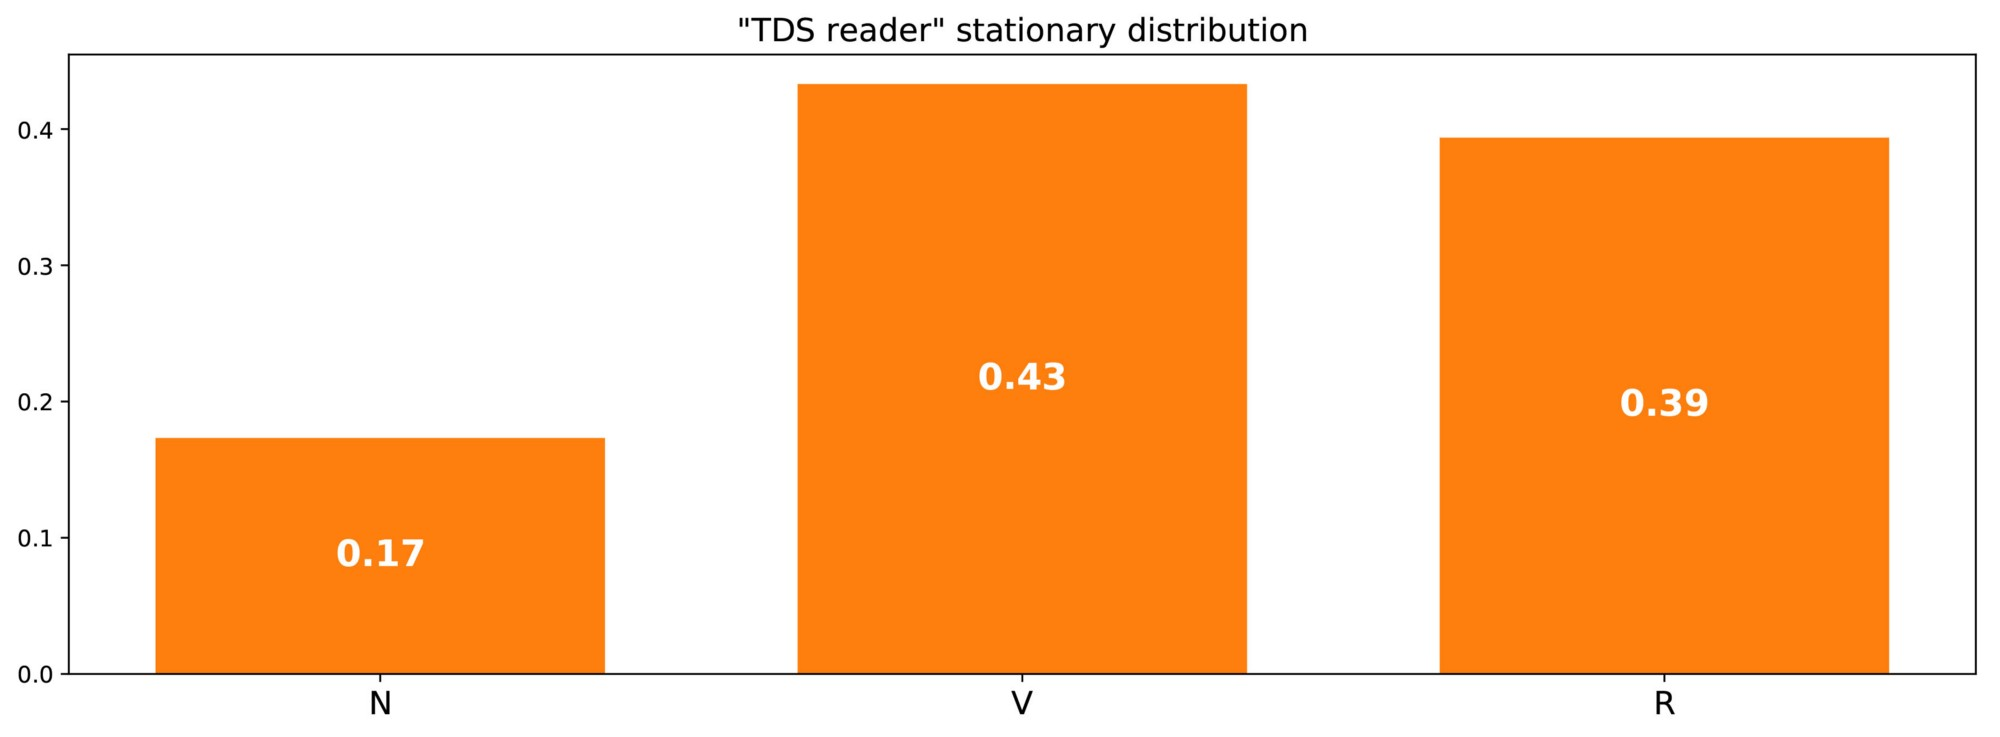
\includegraphics[width=\textwidth]{pic/p05c07-snip08.png}
    \caption{Optimisation process of the Variational Inference approach}
    \label{fig:p05c07-snip08}
\end{figure*}


\section{Takeaways}

The main takeways of this article are:
\begin{itemize}
    \item Bayesian inference is a pretty classical problem in statistics and machine learning that relies on the well known Bayes theorem and whose main drawback lies, most of the time, in some very heavy computations
    \item Markov Chain Monte Carlo (MCMC) methods are aimed at simulating samples from densities that can be very complex and/or defined up to a factor
    \item MCMC can be used in Bayesian inference in order to generate, directly from the "not normalised part" of the posterior, samples to work with instead of dealing with intractable computations
    \item Variational Inference (VI) is a method for approximating distributions that uses an optimisation process over parameters to find the best approximation among a given family
    \item VI optimisation process is not sensitive to multiplicative constant in the target distribution and, so, the method can be used to approximate a posterior only defined up to a normalisation factor
\end{itemize}
    

As already mentioned, MCMC and VI methods have different properties that imply different typical use cases. In one hand, the sampling process of MCMC approaches is pretty heavy but has no bias and, so, these methods are preferred when accurate results are expected, without regards to the time it takes. In the other hand, although the choice of the family in VI methods can clearly introduce a bias, it comes along with a reasonable optimisation process that makes these methods particularly adapted to very large scale inference problem requiring fast computations.

Additional comparisons between MCMC and VI can be found in the excellent Variational Inference: A Review For Statisticians \cite{BleiVariational2017}, that we also highly recommend for readers interested in VI only. For further readings about MCMC, we recommend this general introduction \cite{BrooksHBMonteCarlo2011} as well as this machine learning oriented introduction \cite{Andrieu2003}. The reader interested to learn more about Gibbs Sampling applied to LDA can refer to this Tutorial \cite{Darling2011ATA} on Topic Modelling and Gibbs Sampling (combined with these lecture note \cite{Mukherjee2014} on LDA Gibbs Sampler for cautious derivation).

